\documentclass[11pt]{article}
\usepackage{std}

\title{COMP4680 Notes}
\author{Advanced Topics in Machine Learning: Optimization}
\date{2023 S2}

\begin{document}

\maketitle

\setcounter{section}{-1}
\section{Introduction} 
A mathematical optimisation problem requires us to minimize an objective function $f_0(x)$, subject to constraint functions $f_i(x) \leq b_i$ for $i = 1, \ldots, m$. \par
A solution, or optimal point, $x^*$, has the smallest value of $f_0$ among all vectors that satisfy the constraints. \par 
There are three main types of problems which can be solved to different extents: 
\subsection{Least-squares Problems} 
Least-squares problems attempt to minimize $\norm{Ax - b}_2^2$ for some matrix $A$ and vector $b$. \par
There exists an analytical solution $x^* = (A^TA)^{-1}A^Tb$, there are reliable and efficient algorithms with computation time $O(n^2k)$ when $A \in \mathbb{R}^{k\times n}$, less if $A$ satisfies certain structures. 
\subsection{Convex Optimization Problems} 
Convex optimization problems are optimization problems where both the objective and constraint functions are convex, and is a superset of least-squares problems. \par 
There is no analytical solution, but there are algorithms with computation time $\mathrm{max}(O(n^3), \\O(n^2m), F)$ where $F$ is the cost of evaluating $f_i$'s and their second derivatives. 
\subsection{Nonconvex Optimization Problems} 
There is no general way to solve nonconvex optimization problems: they all involve some kind of compromise. \par
We may use local optimization methods (nonlinear programming), which is fast and finds a local minima around an initial guess, but may not be the global minima. \par
Or we may use global optimization methods, which finds the global solution but requires exponential time complexity. 

\newpage


\section{Preliminaries} 
\subsection{Sets}
A set, denoted as $S = \left\{ a_1, \ldots, a_n \right\}$, is a collection of distinct objects. \par
Some common notations: 
\begin{itemize}
    \item $a \in S$ denotes $a$ is an element of $S$
    \item $S \subseteq T$ denotes $S$ is a subset of $T$, that is, every element of $S$ is also an element of $T$
    \item $S \cup T$ denotes the union of $S$ and $T$, that is, the set of all elements that are in $S$ or $T$
    \item $S \cap T$ denotes the intersection of $S$ and $T$, that is, the set of all elements that are in both $S$ and $T$
    \item $S \times T$ denotes the Cartesian product of $S$ and $T$, that is, the set of all ordered pairs $(s, t)$ where $s \in S$ and $t \in T$
    \item $S \setminus T$ denotes the set difference of $S$ and $T$, that is, the set of all elements that are in $S$ but not in $T$
\end{itemize}  
Some common sets: 
\begin{itemize}
    \item $\mathbb{R}$ is the set of real numbers
    \item $\mathbb{R}^n$ is the set of $n$-dimensional real vectors
    \item $\mathbb{R}^{m\times n}$ is the set of $m \times n$ real matrices
    \item $\mathbb{C}$ is the set of complex numbers
    \item $\mathbb{Z}$ is the set of integers
    \item $\mathbb{R}_+$ is the set of nonnegative real numbers
    \item $\mathbb{R}_{++}$ is the set of positive real numbers
    \item $\emptyset$ is the empty set 
    \item $[a, b]$ is the closed interval from $a$ to $b$ (i.e. $\left\{ x \in \mathbb{R} \mid a \leq x \leq b \right\}$)
    \item $(a, b)$ is the open interval from $a$ to $b$ (i.e. $\left\{ x \in \mathbb{R} \mid a < x < b \right\}$)
    \item $[a, b)$ and $(a, b]$ are half-open intervals, defined similarly
\end{itemize}

\subsubsection*{Open and Closed Sets}
A subset $S \subseteq \mathbb{R}$ is \textbf{open} if for every $x \in S$, there exists $\epsilon > 0$ such that \\
\-\quad if $\norm{y - x}_2 < \epsilon$, then $y \in S$. \par
A subset $S \subseteq \mathbb{R}$ is \textbf{closed} if its complement $\mathbb{R} \setminus S$ is open. \par
A subset $S \subseteq \mathbb{R}$ is \textbf{bounded} if there exists $M > 0$ such that $\norm{a-b}_2 \leq M$ for all $a, b \in S$. \par

\subsubsection*{Infimum and Supremum}
The \textbf{infimum} of a set $S \subseteq \mathbb{R}$, written as $\mathrm{inf}(S)$, is the largest $y \in \mathbb{R}$ such that $y \leq x$ for all $x \in S$. If no such $y$ exists, we say $\mathrm{inf}(S) = -\infty$. \par
The \textbf{supremum} of a set $S \subseteq \mathbb{R}$, written as $\mathrm{sup}(S)$, is the smallest $y \in \mathbb{R}$ such that $y \geq x$ for all $x \in S$. If no such $y$ exists, we say $\mathrm{sup}(S) = \infty$. \par
We define $\mathrm{inf}(\emptyset) = \infty$ and $\mathrm{sup}(\emptyset) = -\infty$. \par 

\subsection{Functions} 
A function $f: A \rightarrow B$ is a mapping from its \textbf{domain} $A$ to its \textbf{codomain} $B$. \par
If $U \subseteq A$ and $V \subseteq B$, we define the \textbf{image} of $U$ under $f$ as $f(U) = \left\{ f(x) \mid x \in U \right\} \subseteq B$, and the \textbf{preimage} of $V$ under $f$ as $f^{-1}(V) = \left\{ x \in A \mid f(x) \in V \right\} \subseteq A$. \par

\subsection{Vector Spaces} 
A vector space $V$ is a set with two operations, vector addition and scalar multiplication, that satisfy the following axioms: 
\begin{itemize}
    \item $x + y = y + x$ (commutativity of vector addition)
    \item $(x + y) + z = x + (y + z)$ (associativity of vector addition)
    \item $x + \vec{0} = x$ (additive identity)
    \item $\forall x \in V, \exists y \in V$ such that $x + y = 0$, we write $y$ as $-x$ (additive inverse)
    \item $\alpha(x + y) = \alpha x + \alpha y$ (right distributivity)
    \item $(\alpha + \beta)x = \alpha x + \beta x$ (left distributivity)
    \item $1x = x$ (multiplicative identity)
\end{itemize}
We define the \textbf{zero vector} as a vector with all elements equal to 0, and the \textbf{ones vector} as a vector with all elements equal to 1. 

\subsubsection*{Euclidean Norm}
The Euclidean norm of a vector $\vec{v} = (v_1, \ldots, v_n)$ is 
\[ \norm{\vec{v}}_2 = \sqrt{v_1^2 + v_2^2 + \cdots + x_n^2} \] 
$\norm{\vec{v}}_2$ measures the length of $\vec{v}$. \par 
The norm satisfies: 
\begin{itemize}
    \item $\norm{\alpha\vec{v}} = \abs{\alpha}\norm{\vec{v}}$
    \item $\norm{\vec{u} + \vec{v}} \leq \norm{\vec{u}} + \norm{\vec{v}}$ (triangle inequality)
    \item $\norm{\vec{v}} \geq 0$ and $\norm{\vec{v}} = 0$ if and only if $\vec{v} = \vec{0}$ (positive definiteness)
\end{itemize}
There are other norms such as $\norm{\phantom{~.~}}_1$ and $\norm{\phantom{~.~}}_\infty$. 

\subsubsection*{Inner Products}
The inner product of two vectors $\vec{u} = (u_1, \ldots, u_n)$ and $\vec{v} = (v_1, \ldots, v_n)$ is defined by 
\[ \langle \vec{u}, \vec{v} \rangle = u_1v_1 + u_2v_2 + \cdots + u_nv_n. \] 
The inner product satisfies:
\begin{itemize}
    \item $\langle \alpha\vec{u}, \vec{v} \rangle = \alpha\langle \vec{u}, \vec{v} \rangle$
    \item $\langle \vec{u}_1 + \vec{u}_2, \vec{v} \rangle = \langle \vec{u}_1, \vec{v} \rangle + \langle \vec{u}_2, \vec{v} \rangle$
    \item $\langle \vec{u}, \vec{v} \rangle = \langle \vec{v}, \vec{u} \rangle$
    \item $\langle \vec{v}, \vec{v} \rangle = \norm{\vec{v}}_2^2$
\end{itemize}

\subsubsection*{Subspaces} 
A subspace of a vector space is a subset of the vector space that is also a vector space. \par
\subsubsection*{Independence}
A set of vectors $v_1, \ldots, v_n$ is (linearly) independent if and only if $\alpha_1v_1 + \cdots + \alpha_nv_n = 0$ implies $\alpha_1 = \cdots = \alpha_n = 0$. \par 
Conversely, if a set of vectors is linearly dependent, we can write one of the vectors as a linear combination of the others. \par
\subsubsection*{Bases}
The set of vectors $\left\{ v_1, \ldots, v_n \right\}$ form a basis of a vector space $V$ if 
\begin{itemize}
    \item they are linearly independent
    \item they span $V$, that is, every vector in $V$ can be written as a linear combination of the vectors in the set
\end{itemize}  
Equivalently, $\left\{ v_1, \ldots, v_n \right\}$ form a basis for $V$ if every $v \in V$ can be uniquely expressed as $v = \alpha_1v_1 + \cdots + \alpha_nv_n$. \par
We define the \textbf{dimension} of a vector space $V$ to be the number of vectors in any basis of $V$. \par
The standard basis of $\mathbb{R}^n$ is the set of vectors $\left\{ e_1, \ldots, e_n \right\}$ where $e_i$ is the vector with a 1 in the $i$\textsuperscript{th} position and 0 elsewhere. \par

\subsection{Matrices} 
A matrix $A \in \mathbb{R}^{m\times n}$ is a rectangular array of real numbers with $m$ rows and $n$ columns. \par
We write $A_{ij}$ for the entry in the $i$\textsuperscript{th} row and $j$\textsuperscript{th} column of $A$. \par
A $n \times 1$ matrix is called a (column) \textbf{vector}, and a $1 \times n$ matrix is called a row \textbf{vector}. \par 

We say a matrix is \textbf{diagonal} if its nonzero entries are all on the main diagonal (top left to bottom right). \par
The \textbf{zero matrix}, denoted $\bm{0}_{m\times n}$, is the matrix with all entries equal to zero. \par
The \textbf{identity matrix}, denoted $\bm{I}_n$, is the $n \times n$ matrix with ones on the main diagonal and zeros elsewhere. \par

\subsubsection*{Special Types of Matrices}
A matrix is \textbf{triangular} if all its entries above or below the main diagonal are zero. In particular, we refer to a matrix as \textbf{upper triangular} if all its entries below the main diagonal are zero, and \textbf{lower triangular} if all its entries above the main diagonal are zero. \par
A matrix is \textbf{block diagonal} if it is diagonal and each diagonal entry is itself a matrix. \par
A matrix is \textbf{tri-diagonal} if it has nonzero entries only on the main diagonal and the diagonals immediately above and below the main diagonal. \par

\begin{figure}[H]
    \centering
    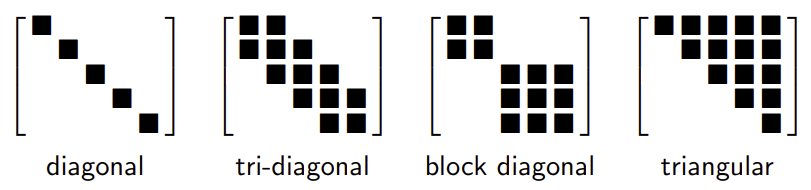
\includegraphics[width=.6\textwidth]{images/1.1}
\end{figure}

\subsubsection*{Matrix Transpose}
Transpose, denotes as $^T$, flips a matrix over is main diagonal, i.e. if $A$ is an $m \times n$ matrix then $A^T$ is an $n \times m$ matrix. It satisfies the following properties: 
\begin{itemize}
    \item $(A^T)^T = A$
    \item $(AB)^T = B^TA^T$
    \item $(A+B)^T = A^T + B^T$
\end{itemize}
If a matrix $A$ satisfies $A = A^T$ we say $A$ is \textbf{symmetric}. \par 
If a matrix $A$ satisfies $A = -A^T$ we say $A$ is \textbf{anti-symmetric}. \par 
Every square matrix $A$ can be written as the sum of a symmetric part and an anti-symmetric part: 
\[ A = \underbrace{\frac{1}{2}\left( A + A^T \right)}_{\text{symmetric}} + \underbrace{\frac{1}{2}\left( A - A^T \right)}_{\text{anti-symmetric}} \] 

\subsubsection*{Notation for Symmetric Matrices} 
We write 
\begin{itemize}
    \item $\mathbb{S}^n$ for the set of symmetric $n\times n$ matrices
    \item $\mathbb{S}^n_+ = \left\{ X \in \mathbb{S}^n \mid X \preceq 0 \right\}$ for the positive semi-definite $n\times n$ matrices  
    \[ X \in \mathbb{S}^n_+ \Leftrightarrow z^TXz \geq 0 \text{ for all } z. \] 
    \item $\mathbb{S}^n_{++} = \left\{ X \in \mathbb{S}^n \mid X \prec 0 \right\}$ for the positive definite $n\times n$ matrices 
\end{itemize}

\subsubsection*{Matrix Addition}
Two matrices of the same size can be added together: we simply add the corresponding elements in each matrix. 

\subsubsection*{Matrix Multiplication}
The product of two matrices $A \in \mathbb{R}^{m\times n}$ and $B \in \mathbb{R}^{n \times p}$ is an $m \times p$ matrix with elements 
\[ C_{ij} = \sum\limits_{k=1}^n A_{ik}B_{kj}. \] 

Matrix multiplication satisfies:
\begin{itemize}
    \item $(AB)C = A(BC)$ (associativity)
    \item $A(B+C) = AB + AC$ (left distributivity)
    \item $(A+B)C = AC + BC$ (right distributivity)
\end{itemize}
but matrix multiplication is not commutative: $AB \neq BA$ generally. \par 

\subsubsection*{Null Space}
The null space of a matrix $A \in \mathbb{R}^{m\times n}$ is defined as 
\[ \mathcal{N}(A) = \left\{ x \in \mathbb{R}^n \mid Ax = 0 \right\}. \] 
$\mathcal{N}(A)$ can be interpreted as
\begin{itemize}
    \item the set of all vectors mapped to zero by $y = Ax$
    \item the set of all vectors orthogonal to the rows of $A$
\end{itemize}
\subsubsection*{Range Space} 
The range space of a matrix $A \in \mathbb{R}^{m\times n}$ is defined as 
\[ \mathcal{R}(A) = \left\{ Ax \mid x \in \mathbb{R}^n \right\} \subseteq \mathbb{R}^m. \] 
$\mathcal{R}(A)$ can be interpreted as 
\begin{itemize}
    \item the set of all vectors that can be ``hit'' by $y = Ax$
    \item the span of the columns of $A$
    \item the set of all vectors $y$ such that $Ax = y$ has a solution
\end{itemize}

\subsubsection*{Orthogonal Complement}
The orthogonal complement of $V \subseteq \mathbb{R}^n$ is defined as 
\[ V^\perp = \left\{ x \mid z^Tx = 0 \text{ for all }  z\in V \right\}. \] 
We have $V \oplus V^\perp = \mathbb{R}^n$. \par

A result from the Fundamental Theorem of Linear Algebra states that $\mathcal{N}(A) = \mathcal{R}(A^T)^\perp$.

\subsubsection*{Rank}
The rank of a matrix $A \in \mathbb{R}^{m\times n}$ is 
\[ \mathrm{rank}(A) = \dim \mathcal{R}(A). \] 

\begin{itemize}
    \item $\mathrm{rank}(A) = \mathrm{rank}(A^T)$ 
    \item $\mathrm{rank}(A)$ is the maximum number of independent columns (or rows) of $A$. Hence $\mathrm{rank}(A) \leq \mathrm{min}\{m, n\}$. 
    \item $\mathrm{rank}(A) + \mathrm{dim}\mathcal{N}(A) = n$ (rank-nullity)
\end{itemize}
We say a matrix $A$ is \textbf{full rank} if $\mathrm{rank}(A) = \mathrm{min}\{m, n\}$. \par

The rank of the product of two matrices satisfies 
\[ \mathrm{rank}(AB) \leq \min\left\{ \mathrm{rank}(A), \mathrm{rank}(B) \right\}. \] 
If $A \in \mathbb{R}^{m\times n}$ has rank $r$ then $A$ can be factored as $BC$ with $B \in \mathbb{R}^{m\times r}$ and $C \in \mathbb{R}^{r \times n}$. 

\subsubsection*{Trace}
The trace of a square matrix $A \in \mathbb{R}^{n\times n}$ is the sum of its diagonal entries, i.e. 
\[ \mathrm{tr}(A) = \sum_{j=1}^n A_{jj}. \] 
Trace satisfies the following properties: 
\begin{itemize}
    \item $\mathrm{tr}(A) = \mathrm{tr}(A^T)$
    \item $\mathrm{tr}(\alpha A + \beta B) = \alpha\mathrm{tr}(A) + \beta\mathrm{tr}(B)$
    \item if $AB$ is square then $\mathrm{tr}(AB) = \mathrm{tr}(BA)$
\end{itemize}

\subsubsection*{Determinant}
The determinant of a square matrix $A \in \mathbb{R}^{n\times n}$ is a function $\det: \mathbb{R}^{n\times n} \rightarrow \mathbb{R}$ that satisfies the following properties:
\begin{itemize}
    \item $\det \bm{I} = 1$
    \item $\det \alpha A = \alpha^n \det A$
    \item swapping any two rows/columns changes the sign of the determinant 
    \item $\det AB = \det A \det B$
\end{itemize} 
We can interpret the determinant as the volume of the parallelepiped spanned by the rows (or columns) of $A$. \par

\subsubsection*{Matrix Inverse} 
The inverse of a square matrix $A \in \mathbb{R}^{n\times n}$ is a matrix $A^{-1}$ such that 
\[ AA^{-1} = A^{-1}A = \bm{I} \] 
A matrix is \textbf{invertible} (i.e. has an inverse) if and only if $\det A \neq 0$. This is equivalent to: 
\begin{itemize}
    \item the columns/rows of $A$ form a basis for $\mathbb{R}^n$
    \item $y = Ax$ has a unique solution for all $x \in \mathbb{R}^n$
    \item $A$ is full-rank (i.e. $\mathcal{N}(A) = \{ 0 \}$ and $\mathcal{R}(A) = \mathbb{R}^n$)
    \item $\det A^TA = \det AA^T \neq 0$
\end{itemize}

\subsubsection*{Cauchy-Schwarz Inequality}
For any vectors $x, y \in \mathbb{R}^n$, we have that 
\[ \abs{x^Ty} \leq \norm{x}_2 \norm{y}_2. \] 
The angle between vectors in $\mathbb{R}^n$ is given by 
\[ \theta = \cos^{-1}\left( \frac{x^Ty}{\norm{x}_2\norm{y}_2} \right). \] 
\begin{itemize}
    \item If $x$ and $y$ are aligned then $x^Ty = $
\end{itemize}

\subsubsection*{Eigenvalues and Eigenvectors}
$\lambda \in \mathbb{C}$ is an eigenvalue of $A \in \mathbb{R}^{n\times n}$ if 
\[ \det(\lambda I - A) = 0. \] 
Equivalently, there exists a non-zero $v \in \mathbb{C}^n$ such that $(\lambda I - A)v = 0$, or $Av = \lambda v$. Any such $v$ here is called an eigenvector of $A$, associated with eigenvalue $\lambda$. \par 
The eigenvalues of a symmetric matrix $A \in \mathbb{R}^{n\times n}$ are real. Moreover, there exists a set of orthogonal eigenvectors $q_1, \ldots, q_n$ such that $Aq_i = \lambda_iq_i$ and $q_i^Tq_j = 0$ if $i \neq j$. \par 
In matrix form, there is an orthonormal $Q$ such that $A = Q\Lambda Q^T$.

\subsubsection*{Norm Matrices}
A matrix norm is a function $\norm{\phantom{~.~}}: \mathbb{R}^{m\times n} \rightarrow \mathbb{R}$ that, similar to vector norms, satisfy linearity, positive definiteness, and the triangle inequality. \par
\begin{itemize}
    \item Induced norms: $\norm{A} = \sup \left\{ \norm{Ax} \mid x \in \mathbb{R}^n, \norm{x} \leq 1 \right\}$
    \item Frobenius norm: $\norm{A}_F = \sqrt{\left\{ \sum_{ij} a_{ij}^2 \right\}}$
    \item Nuclear norm: $\norm{A}_* = \sum_i \sigma_i(A) = \mathrm{tr}(\sqrt{A^TA})$  
\end{itemize} 
Square matrices also satisfy the sub-multiplicative property: 
\[ \norm{AB} \leq \norm{A}\norm{B}. \] 

\subsection{Matrix Factorization} 
\subsubsection*{LU Factorization} 
Every nonsingular matrix $A \in \mathbb{R}^{n\times n}$ can be factored as 
\[ A = PLU \] 
where $P$ is a permutation matrix, $L$ is unit lower triangular, and $U$ is upper triangular and non-singular. 
\subsubsection*{Cholesky Factorization} 
Every symmetric positive definite matrix $A \in \mathbb{R}^{n\times n}$ can be factored as 
\[ A = LL^T \] 
where $L$ is lower triangular and non-singular with positive diagonal elements. 
\subsubsection*{Singular Value Decomposition} 
Any matrix $A$ can be decomposed as 
\[ A = U\Sigma V^T \] 
where $A \in \mathbb{R}^{m\times n}$ has rank $r$, $U \in \mathbb{R}^{m\times r}$, $V \in \mathbb{R}^{n\times r}$ which satisfy $U^TU = I$ and $V^TV = I$, and $\Sigma = \mathrm{diag}(\sigma_1, \ldots, \sigma_r)$ with $\sigma_1 \geq \sigma_2 \geq \cdots \geq \sigma_r > 0$. \par 
Since $A^TA = V\Sigma^2V^T$ we have $v_i$ are the eigenvectors of $A^TA$. Similarly, $u_i$ are the eigenvectors of $AA^T$. \par 
We can use SVD to interpret a linear map $y = Ax$ as follows: 
\begin{itemize}
    \item we compute coefficients of $x$ along the input directions $v_1, \ldots, v_r$
    \item scale the coefficients by $\sigma_i$
    \item re-constitute along the output directions $u_1, \ldots, u_r$
\end{itemize}
Here, $v_1$ is the most sensitive input direction, and $u_1$ is the highest gain output direction. 

\subsubsection*{Matrix Calculus}
We can compute partial derivatives of a function $f: \mathbb{R}^{m\times n} \rightarrow \mathbb{R}$ as 
\[ \pp[f(x)]{x_{ij}} = \lim_{\alpha \rightarrow 0} \frac{f(x + \alpha e_ie_j^T) - f(x)}{\alpha}. \] 
We can also compute the gradient (Jacobian) of $f$ as 
\[ \nabla_Af(A) = \begin{pmatrix}
    \pp[f]{A_{11}} & \pp[f]{A_{12}} & \ldots & \pp[f]{A_{1n}} \\
    \pp[f]{A_{21}} & \pp[f]{A_{22}} & \ldots & \pp[f]{A_{2n}} \\
    \vdots & \vdots & \ddots & \vdots \\
    \pp[f]{A_{m1}} & \pp[f]{A_{m2}} & \ldots & \pp[f]{A_{mn}} 
\end{pmatrix} \] 
Partial derivatives are linear: 
\begin{itemize}
    \item $\nabla_A(f + g) = \nabla_Af + \nabla_Ag$
    \item $\nabla_A(tf) = t\nabla_Af$
\end{itemize}
Chain rule and product rule also extend to matrix calculus. \par 
In vector calculus, the \textbf{Hessian} of a function $f: \mathbb{R}^n \rightarrow \mathbb{R}$ is the matrix of second-order partial derivatives of $f$, i.e. 
\[ \nabla_x^2 f(x) = \begin{pmatrix} 
    \pn*[f]{2}{x_1^2} & \pn*[f]{2}{x_1x_2} & \ldots & \pn*[f]{2}{x_1x_n} \\
    \pn*[f]{2}{x_2x_1} & \pn*[f]{2}{x_2^2} & \ldots & \pn*[f]{2}{x_2x_n} \\
    \vdots & \vdots & \ddots & \vdots \\
    \pn*[f]{2}{x_nx_1} & \pn*[f]{2}{x_nx_2} & \ldots & \pn*[f]{2}{x_n^2}
\end{pmatrix} \]  

\subsection{Probability Theory} 
A probability distribution is a function that maps outcomes of an experiment to probabilities: 
\begin{itemize}
    \item for discrete variables we have \textbf{probability mass functions} 
    \item for continuous variables we have \textbf{probability density functions} 
\end{itemize}
The \textbf{mean} or \textbf{expected value} of a random variable is the sum of possible values weighted by their probabilities: 
\[ \mathbb{E}[X] = \int_x x P(X = x) \di{x} \] 
The \textbf{variance} of a random variable $X$ is $\mathbb{E}[(X - \mathbb{E}[X])^2]$. \par 

\subsection{Geometric Concepts} 
\subsubsection*{Lines} 
A line through two points $x_1$ and $x_2$ has the equation $x = \theta x_1 + (1 - \theta) x_2$. \par 
The \textbf{line segment} between $x_1$ and $x_2$ is the set of points $x = \theta x_1 + (1 - \theta) x_2$ for $0 \leq \theta \leq 1$. \par

\subsubsection*{Affine Sets} 
An affine set contains the line through any two distinct points in the set: if $x_1, x_2 \in S$ then $\theta x_1 + (1-\theta) x_2 \in S$. \par 
Every affine set can be expressed as the solution set of a system of linear equations. 

\subsubsection*{Convex Sets} 
A convex set contains the line segment between any two distinct points in the set: if $x_1, x_2 \in S$ then $\theta x_1 + (1-\theta) x_2 \in S$ for $0 \leq \theta \leq 1$. \par
Common examples: 
\begin{itemize}
    \item nonnegative orthant: $\mathbb{R}_+^n$ = $\left\{ x \in \mathbb{R}^n \mid x_i \geq 0 \right\}$
    \item positive semidefinite matrices: $\mathbb{S}_+^n = \left\{ X \in \mathbb{R}^{n\times n} \mid z^TXz \geq 0, z \in \mathbb{R}^n \right\}$
\end{itemize}

\subsubsection*{Convex Combinations and Hulls} 
A convex combination of $x_1, \ldots, x_k$ is any point of the form 
\[ x = \theta_1x_1 + \theta_2x_2 + \ldots + \theta_kx_k \]
where $\theta_1 + \theta_2 + \ldots + \theta_k = 1$ and $\theta_i \geq 0$ for all $i$. \par
The convex hull of a set $S$, $\mathrm{conv}(S)$, is the set of all convex combinations of points in $S$. \par

\subsubsection*{Convex Cones} 
A \textbf{conic combination} of points $x_1$ and $x_2$ is any point of the form 
\[ x = \theta_1 x_1 + \theta_2 x_2 \] 
with $\theta_1, \theta_2 \geq 0$. \par 
A cone is a set containing all non-negative multiples of its points (i.e. if $x \in C$ then $\alpha x \in C$ for all $\alpha \geq 0$). \par
A convex cone is a set containing all conic combinations of its points. 

\subsubsection*{Hyperplanes and Halfspaces} 
A hyperplane is a set of the form $\left\{ x \mid a^Tx = b \right\}$ with $a \neq 0$. \par
A halfspace is a set of the form $\left\{ x \mid a^Tx \leq b \right\}$ with $a \neq 0$. \par
In the 3D case, a plane is a hyperplane while a halfspace is everything on one side of the plane. \par 
Hyperplanes are affine and convex, and halfspaces are convex.

\subsubsection*{Euclidean Balls and Ellipsoids} 
A Euclidean ball with center $x$ and radius $r$ is a set $B(x, r) = \left\{ y \mid \norm{y - x}_2 \leq r \right\}$. \par
An ellipsoid is a set of the form 
\[ \left\{ y \mid (y - x)^T P^{-1} (y - x) \leq 1 \right\} \] 
with $P \in \mathbb{S}_{++}^n$ (symmetric positive definite). \par 
Alternatively, we can represent a ball as 
\[ B(x, r) = \left\{ x + ru \mid \norm{u}_2 \leq 1 \right\} \] 
and an ellipsoid as 
\[ \left\{ x + Au \mid \norm{u}_2 \leq 1 \right\} \] 
with $A$ a square, nonsinguar matrix. 

\subsubsection*{Norm Balls and Cones} 
A norm ball with center $x$ and radius $r$ is the set $\left\{ y \mid \norm{y - x} \leq r \right\}$. \par 
A norm cone is the set $\left\{ (x, t) \mid \norm{x} \leq t \right\}$. 
Norm balls and cones are convex.

\subsubsection*{Polyhedra} 
A polyhedron is the solution set of finitely many linear inequalities and equalities 
\[ Ax \preceq b, Cx = d \] 
where $\preceq$ is componentwise inequality. \par 
So a polyhedron is the intersection of a finite number of halfspaces and hyperplanes. 
Polyhedra are convex sets. 

\subsubsection*{Summary of Convex Sets} 
\begin{figure}[H]
    \centering
    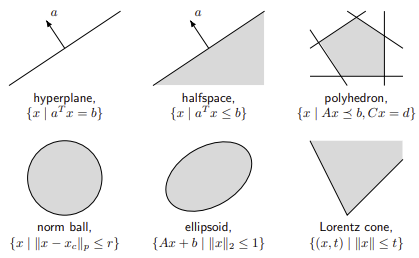
\includegraphics{images/2.1}
\end{figure}

\subsubsection*{Obtaining Convex Sets} 
We can either show a set $C$ is convex by applying the definition, or obtain $C$ using the following properties: 
\begin{itemize}
    \item the intersection of any number of convex sets is convex 
    \item the image of a convex set under an affine map is convex (recall affine maps are of the form $f(x) = Ax + b$)
    \item the preimage of a convex set under an affine map is convex
    \item perspective functions preserve convexity: these are functions of the form 
    \[ P(x, t) = x/t, t > 0 \] 
    \item linear-fractional functions preserve convexity: these are functions of the form 
    \[ f(x) = \frac{Ax + b}{c^Tx + d}, c^Tx + d > 0 \]     
\end{itemize}

\subsubsection*{Generalized Inequalities} 
A convex cone $K \subseteq \mathbb{R}^n$ is a \textbf{proper cone} if 
\begin{itemize}
    \item $K$ is closed (contains its boundary)
    \item $K$ is solid (has nonempty interior)
    \item $K$ is pointed (contains no line)
\end{itemize}
Examples include, 
\begin{itemize}
    \item the nonnegative orthant
    \item positive semidefinite cone $\mathbb{S}_+^n$
    \item nonnegative polynomials on $[0, 1]$ 
    \[ K = \left\{ x \in \mathbb{R}^n \mid x_0 + x_1t + x_2t^2 + \cdots + x_nt^n \geq 0, t \in [0, 1] \right\} \] 
\end{itemize}

A generalized inequality is a relation of the form 
\[ x \preceq_K y \Leftrightarrow y - x \in K \] 
and 
\[ x \prec_K y \Leftrightarrow y - x \in \mathrm{int}(K) \] 
where $\mathrm{int}(K)$ denotes the interior of $K$. \par 
\begin{itemize}
    \item In the case of the nonnegative orthant $K = \mathbb{R}^n_+$, we have componentwise inequality $x \preceq y \Leftrightarrow x_i \leq y_i$ for all $i$. 
    \item In the case of the positive semidefinite cone $K = \mathbb{S}_+^n$, we have $X \preceq Y \Leftrightarrow Y - X \in \mathbb{S}_+^n$.
\end{itemize}
In these cases, we omit the subscript $K$ and write $x \preceq y$ and $X \preceq Y$. \par

\subsubsection*{Minimum and Minimal Elements} 
As $\preceq$ is not a linear order, we have to define 
\begin{itemize}
    \item $x \in S$ is the minimum element of $S$ with respect to $\preceq$ if $x \preceq y$ for all $y \in S$
    \item $x \in S$ is the minimal element of $S$ with respect to $\preceq$ if there is no $y \in S$ such that $y \prec x$
\end{itemize}

\subsubsection{Separating Hyperplane Theorem} 
If $C$ and $D$ are nonempty disjoint convex sets, there exists $a \neq 0, b$ such that 
\[ a^Tx \leq b \text{ for } x \in C, \quad, a^Tx \geq b \text{ for } x \in D \] 
That is, there exists a hyperplane separating any two convex sets $C$ and $D$. (Strict separation requires additional assumptions, e.g. $C$ is closed, $D$ is singleton)
\subsubsection*{Supporting Hyperplane Theorem} 
A supporting hyperplane to a set $C$ at a boundary point $x_0$ is 
\[ \left\{ x \mid a^Tx = a^Tx_0 \right\}  \] 
where $a \neq 0$ and $a^T \leq a^Tx_0$ for all $x \in C$. \par
This can be thought of as a tangent hyperplane. \par 
The theorem states that there exists a supporting hyperplane at any point on the boundary of a convex set. \par 

\subsubsection*{Dual Cones and Generalized Inequalities}
The dual cone of a cone $K$ is 
\[ K^* = \left\{ y \mid y^Tx \geq 0 \text{ for all } x \in K \right\} \] 
Examples: 
\begin{itemize}
    \item For $K = \mathbb{R}^n_+$, we have $K^* = \mathbb{R}^n_+$
    \item For $K = \mathbb{S}_+^n$, we have $K^* = \mathbb{S}_+^n$
    \item For $K = \left\{ (x, t) \mid \norm{x}_2 \leq t \right\}$, we have $K^* = \left\{ (x, t) \mid \norm{x}_2 \leq t \right\}$ 
    \item For $K = \left\{ (x, t) \mid \norm{x}_1 \leq t \right\}$, we have $K^* = \left\{ (x, t) \mid \norm{x}_\infty \leq t \right\}$ 
\end{itemize}
We say a cone is self-dual if it is its own dual. \par 
Dual cones of proper cones are proper, hence defining generalized inequalities: 
\[ y \succeq_{K^*} 0 \Leftrightarrow y^Tx \geq 0 \text{ for all } x \succeq_K 0 \] 

We can define minimum and minimal elements using these dual inequalities: 
\begin{itemize}
    \item $x$ is the minimum element of $S$ iff for all $\lambda \succ_{K^*} 0$, $x$ is the unique minimizer of $\lambda^Tz$ over $S$
    \item $x$ is a minimal element of $S$ if it minimizes $\lambda^Tz$ for some $\lambda \succ_{K^*} 0$
    \item if $x$ is a minimal element of a convex set $S$, then there exists a nonzero $\lambda \succeq_{K^*} 0$ such that $x$ minimizes $\lambda^Tz$ over $S$
\end{itemize}

\newpage
\section{Convex Functions} 
A function $f: \mathbb{R}^n \rightarrow \mathbb{R}$ is convex if $\mathrm{dom} f$ is convex and 
\[ f(\theta x + (1 - \theta)y) \leq \theta f(x) + (1-\theta) f(y) \] 
for all $x, y \in \mathrm{dom} f$ and $0 \leq \theta \leq 1$. \par

\begin{itemize}
    \item $f$ is concave if $-f$ is convex
    \item $f$ is strictly convex if the inequality holds strictly
    \item $f$ is strongly convex if it has minimum positive curvature everywhere
\end{itemize}
For example, all affine functions and norms on $\mathbb{R}^n$ are convex. \par 

A function $f: \mathbb{R}^n \rightarrow \mathbb{R}$ is convex if and only if the function $g: \mathbb{R} \rightarrow \mathbb{R}$ defined by $g(t) = f(x+tv)$ is convex for any $x \in \mathrm{dom} f$, $v \in \mathbb{R}^n$. That is, a function $f$ is convex if and only if it is convex on every line.

\subsection{Extended-value Extension} 
The extended-value extension $\tilde{f}$ of $f$ is 
\[ \tilde{f}(x) = \begin{cases} 
    f(x), & x \in \mathrm{dom}f \\
    \infty, & x \notin \mathrm{dom}
\end{cases}. \] 
This simplifies our definition of convexity, the requirement that the domain is convex is no longer needed.

\subsection{First-order condition} 
$f$ is differentiable if $\mathrm{dom} f$ is open and the gradient 
\[ \nabla f(x) = \left( \pp[f(x)]{x_1}, \pp[f(x)]{x_2}, \ldots, \pp[f(x)]{x_n} \right) \] 
exists at each $x \in \mathrm{dom} f$. \par 
If $f$ is differentiable with convex domain, $f$ is convex iff 
\[ f(y) \geq f(x) + \nabla f(x)^T(y-x) \text{ for all } x, y \in \mathrm{dom}f. \] 
(First-order/linear approximation is an underestimate)

\subsection{Second-order conditions} 
$f$ is twice differentiable if $\mathrm{dom}f$ is open and the hessian $\nabla^2 f(x) \in \mathbb{S}^n$ 
\[ \nabla^2 f(x)_{ij} = \frac{\partial^2 f(x)}{\partial x_i \partial x_j} \] 
exists at each $x \in \mathrm{dom}f$ for $i,j = 1, \ldots, n$. \par 
If $f$ is twice differentiable with convex domain, $f$ is convex iff $\nabla^2 f(x) \succeq 0$ for all $x \in \mathrm{dom}f$. \par
Furthermore, if $\nabla^2 f(x) \succ 0$ then $f$ is strictly convex, while if $\nabla^2 f(x) \succ nI$ for some $n > 0$, then $f$ is strongly convex. 

\subsection{Epigraph and Sublevel set}
The $\alpha$-sublevel set of $f: \mathbb{R}^n \rightarrow \mathbb{R}$ is 
\[ C_\alpha = \left\{ x \in \mathrm{dom}f \mid f(x) \leq a \right\}. \] 
Sublevel sets of convex functions are convex. \par 
The epigraph of $f: \mathbb{R}^n \rightarrow \mathbb{R}$ is 
\[ \mathrm{epi} f = \left\{ (x, t) \in \mathbb{R}^{n+1} \mid f(x) \leq t \right\}. \] 
$f$ is convex iff $\mathrm{epi}f$ is convex. 

\subsection{Jensen's Inequality} 
If $f$ is convex, then 
\[ f(\mathbb{E}[z]) \leq \mathbb{E}[f(z)] \] 
for any random variable $z$. \par 
When $z$ is a point distribution at $x$ and $y$, we obtain our convexity condition 
\[ f(\theta x + (1-\theta) y) \leq \theta f(x) + (1-\theta)f(y). \] 

\subsection{Obtaining Convex Functions} 
We can show a function $f$ is convex using the definition, by applying some conditions above, or use the following properties: 
\begin{itemize}
    \item $\alpha f$ is convex if $f$ is convex with $\alpha \geq 0$ 
    \item if $f_1, f_2$ are convex, $f_1 + f_2$
    \item $f(Ax+b)$ is convex if $f$ is convex
    \item if $f_1, f_2$ are convex, $\mathrm{max}(f_1, f_2)$ is convex
    \item if $f(x, y)$ is convex, $\mathrm{sup}_y f(x, y)$ is convex
    \item if $g, h$ are convex and $\tilde{h}$ is nondecreasing in each argument, $h \circ g$ is convex
    \item if $f(x, y)$ is convex and $C$ is convex, $\mathrm{inf}_{y \in C} f(x, y)$ is convex
    \item if $f$ is convex, $g(x, t) = tf(x/t)$ is convex
\end{itemize}

\subsection{The Conjugate Function} 
The conjugate of a function $f$ is 
\[ f^*(y) = \mathrm{sup}_x (y^Tx - f(x)). \] 
The conjugate of a function is always convex. 

\subsection{Types of Convexity} 
\subsubsection*{Quasiconvexity} 
A function $f: \mathbb{R}^n \rightarrow \mathbb{R}$ is quasiconvex if $\mathrm{dom}f$ is convex and the sublevel sets 
\[ S_\alpha = \left\{ x \in \mathrm{dom}f \mid f(x) \leq a \right\} \] 
are convex for all $\alpha$. \par 
Alternatively, $f$ satisfies 
\[ f(\theta x + (1-\theta)y) \leq \mathrm{max}\{ f(x), f(y) \}. \] 

We define $f$ as quasiconcave if $-f$ is quasiconvex, and $f$ as quasilinear if it's both quasiconvex and quasiconcave. \par 
First order condition: if $f$ is differentiable with convex domain, $f$ is quasiconvex iff 
\[ f(y) \leq f(x) \Rightarrow \nabla f(x)^T(y-z) \leq 0. \] 

\subsubsection*{Log Convexity} 
A positive function $f$ is log-concave if $\log f$ is concave: 
\[ f(\theta x + (1-\theta) y) \geq f(x)^\theta f(y)^{1-\theta}. \] 
$f$ is log-convex if $\log f$ is convex. \par 

\begin{itemize}
    \item if $f$ is twice differentiable then it is log-concave iff 
    \[ f(x) \nabla^2f(x) \succeq \nabla f(x) \nabla f(x)^T \] 
    for all $x$. 
    \item the product of log-concave functions is log-concave 
    \item if $f: \mathbb{R}^n \times \mathbb{R}^m \rightarrow \mathbb{R}$ is log-concave, then 
    \[ g(x) = \int f(x, y) \di{y} \] 
    is log-concave. (For example, we can apply this to the convolution formula.)
\end{itemize}

\subsubsection*{Convexity with respect to Generalized Inequalities} 
$f: \mathbb{R}^n \rightarrow \mathbb{R}^m$ is $K$-convex if $\mathrm{dom} f$ is convex and 
\[ f(\theta x + (1-\theta)y) \preceq_K \theta f(x) + (1-\theta) f(y). \] 

\newpage 
\section{Convex Optimization} 
Recall: the general optimization problem has the form \\
minimize $f_0(x)$ subject to $f_i(x) \leq 0$ and $h_i(x) = 0$. \par 
The $f_i$ and $h_i$ are called \textbf{explicit constraints}, and introduce \textbf{implicit constraints} restricting $x$ to the domain of each $f_i, h_i$. We say a problem is \textbf{unconstrained} if there are no explicit constraints. \par 

A point $x$ is \textbf{feasible} if $x \in \mathrm{dom} f_0$ and it satisfies the constraints. A \textbf{solution} or \textbf{optimal point}, $x^*$ has the smallest value of $f_0$ among all feasible $x$. \par 
We may also solve \textbf{feasibility problems} where $f_0 = 0$, and our goal is to find any feasible $x$. \par 

The \textbf{optimal value} of the problem is 
\[ p^* = \mathrm{inf}_{x \in \mathrm{dom}f_0} \left\{ f_0(x) \mid f_i(x) \leq 0, h_i(x) = 0 \right\}. \] 
\begin{itemize}
    \item $p^* = f_0(x^*)$ when $x^*$ exists
    \item $p^* = \infty$ if the problem is infeasible
    \item $p^* = -\infty$ if the problem is unbounded below
\end{itemize}

A point $x$ is \textbf{locally optimal} if there is an $R > 0$ such that $z = x$ is optimal with the additional constraint $\norm{z-x}_2 \leq R$. \par 

We say an optimization problem is \textbf{convex} if $f_0, f_i$ are convex and $h_i$ are affine. If the objective function $f_0$ is \textbf{quasiconvex}, we say the problem is quasiconvex. \par 
Any local optimal point of a convex optimization problem is globally optimal.

\subsection{Optimality Criteria} 
If $f_0$ is differentiable, then $x$ is optimal iff $\nabla f_0(x)^T(y-x) \geq 0$ for all feasible $y$. \par 
For example: 
\begin{itemize}
    \item For an unconstrained problem, $x$ is optimal iff $\nabla f_0(x) = 0$
    \item For an equality constrained problem (i.e. subject to $Ax=b$), $x$ is optimal iff $\nabla f_0(x) + A^T\lambda = 0$ for some $\lambda$
    \item If we want to minimize $f_0$ subject to $x \succeq 0$, $x$ is optimal iff $\nabla f_0(x)$ is nonnegative in the $i$-th component when $x_i = 0$ and zero otherwise
\end{itemize}

\subsection{Equivalent Problems} 
Two problems are equivalent if the solution of one is readily obtained from the solution of the other, and vice versa. Some common transformations that preserve convexity are:
\begin{itemize}
    \item Eliminating equality constraints, we can replace an equality constraint $Ax = b$ with the solution $x = Fz + x_0$ where $x_0$ is a particular solution and the columns of $F$ span $\mathcal{N}(A)$. Then, we may write the problem to minimize $f_0(Fz + x_0)$. 
    \item Introducing equality constraints, converse to the above.
    \item Introducing slack variables for linear inequalities, we can replace an inequality constraint $a^Tx \leq b$ with $a^Tx + s = b$ and $s \geq 0$.
    \item Epigraph form, we can replace the objective minimize $f_0(x)$ with minimizing $t$ with constraint $f_0(x) - t \leq 0$. 
    \item Variable reduction, we can replace the problem minimize $f_0(x_1, x_2)$ with minimize $g(x)$ with $g(x) = \mathrm{inf}_{x_2} f_0(x_1, x_2)$.
\end{itemize}

\subsection{Convex representation of Quasiconvex objective function} 
If $f_0$ is quasiconvex, there exists a family of functions $\phi_t$ such that $\phi_t$ is convex in $x$ for fixed $t$, and 
\[ f_0(x) \leq t \Leftrightarrow \phi_t(x) \leq 0. \] 
Then, we can solve a convex feasibility problem,
\[ \phi_t(x) \leq 0, f_i(x) \leq 0, Ax=b \] 
where we can conclude either $t \geq p^*$ (feasible) or $t \leq p^*$ (infeasible). 

\subsubsection*{Chebyshev Center}
The Chebyshev center of 
\[ \mathcal{P} = \left\{ x \mid a_i^Tx \leq b_i \right\} \] 
is the center of the largest inscribed ball 
\[ \mathcal{B} = \left\{ x_c + u \mid \norm{u}_2 \leq r \right\}. \] 


\subsection{Families of Convex optimization problems}
\subsubsection*{Linear Program} 
A linear program is an optimization problem of the form 
\[ \text{minimize } c^Tx \text{ subject to } Gx \preceq h, Ax = b. \]
\begin{itemize}
    \item Convex problem with affine objective and constraint functions 
    \item Feasible set is a polyhedron
    \item There always exists a solution at a vertex
\end{itemize}
For example, the diet problem of minimizing costs $c_j$ of $n$ food each with nutritional value $a_{ij}$ of nutrient $i$, subject to at least $b_i$ of nutrient $i$ has the form 
\[ \text{minimize } c^Tx \text{ subject to } Ax \succeq b. \] 

\subsubsection*{Linear-fractional Program} 
A linear-fractional program is an optimization problem of the form
\[ \text{minimize } \frac{c^Tx + d}{e^Tx + f} \text{ subject to } Gx \preceq h, Ax=b. \]
This is a quasiconvex optimization problem which can be solved by bisection, and equivalent to a linear program 
\[ \text{minimize } c^Ty + dz \text{ subject to } Gy \preceq hz, Ay=bz, e^Ty + fz = 1, z \geq 0. \] 

A generalized linear-fractional program has the form 
\[ f_0(x) = \mathrm{max} \frac{c_i^Tx + d_i}{e_i^Tx + f_i} \] 
which is also a quasiconvex optimization problem and can be solved by bisection.

\subsubsection*{Quadratic Program} 
A quadratic program is an optimization problem of the form 
\[ \text{minimize } \frac{1}{2}x^TPx + q^Tx + r \text{ subject to } Gx \preceq h, Ax=b. \]

For example, least squares and curve fitting are quadratic programs, and so is a linear program with random cost (minimize $\mathbb{E}[c^Tx] + \gamma\mathbb{V}[c^Tx]$ where $\gamma$ is a risk parameter). 

\subsubsection*{Quadratically Constrained Quadratic Program}
A quadratically constrained quadratic program is an optimization problem of the form
\[ \text{minimize } \frac{1}{2}x^TP_0x + q_0^Tx + r_0 \text{ subject to } \frac{1}{2}x^TP_ix + q_i^Tx + r_i \leq 0, i = 1, \ldots, m, Ax=b. \] 

\subsubsection*{Second-order Cone Program}
A second-order cone program is an optimization problem of the form
\[ \text{minimize } f^Tx \text{ subject to } \norm{A_ix + b_i}_2 \leq c_i^Tx + d_i, i = 1, \ldots, m, Fx = g. \] 
where $A_i \in \mathbb{R}^{n_i \times n}, F \in \mathbb{R}^{p \times n}$. \par 
\begin{itemize}
    \item The inequalities are called second-order cone constraints: $(A_ix + b_i, c_i^Tx + d_i)$ is a second-order cone on $\mathbb{R}^{n_i+1}$
    \item When $n_i = 0$, it reduces to LP; if $c_i = 0$ it reduces to QCQP. 
\end{itemize}

\subsubsection*{Robust Linear Programming}
The parameters in optimization problems are often uncertain, there are two common approaches: 
\begin{itemize}
    \item Deterministic model: constraints holds for all $a_i$ in a small neighbourhood around the true value: i.e. the constraints are $a_i^Tx \leq b_i$ for all $a_i \in \mathcal{E}_i$. 
    \item Stochastic model: $a_i$ is a random variable, and the constraints must hold with some probability $\eta$. 
\end{itemize} 

The deterministic model can be converted to a SOCP by defining 
\[ \mathcal{E}_i = \left\{ \obar{a}_i + P_iu \mid \norm{u}_2 \leq 1 \right\}. \] 
Then, we can convert the constraint to $\obar{a}_i^Tx + \norm{P_i^Tx}_2 \leq b_i$. \par 

The stochastic model can be converted to a SOCP by converting the constraint to $\obar{a}_i^Tx + \Phi^{-1}(\eta)\norm{\sigma_ix}_2 \leq b_i$, where $\Phi$ is the standard normal CDF, and $\sigma_i$ is the standard deviation. 

\subsubsection*{Geometric Program}
A \textbf{monomial} function is a function of the form 
\[ f(x) = cx_1^{a_1}x_2^{a_2}\cdots x_n^{a_n} \] 
defined on $\mathbb{R}^n_{++}$. \par
A \textbf{posynomial} function is a sum of monomials. \par 
A geometric program is an optimization problem of the form 
\[ \text{minimize } f_0(x) \text{ subject to } f_i(x) \leq 1, h_i(x) = 1 \] 
with $f_i$ posynomial and $h_i$ monomial. \par 
We can convert geometric programs to convex problems by taking the logarithm of the objective and constraints, and then solving the resulting convex problem.

\subsubsection*{Generalized Inequality Constraints} 
We can have optimization problems with generalized inequality constraints, for example a constraint of the form $f_i(x) \preceq_K 0$ where $K$ is a proper cone. \par
Specifically, the conic form problem has affine objective and constraints takes the form 
\[ \text{minimize } c^Tx \text{ subject to } Fx+g \preceq_K 0, Ax=b \] 
extends linear programming to nonpolyhedral cones.

\subsubsection*{Semidefinite Program}
A semidefinite program is an optimization problem of the form 
\[ \text{minimize } c^Tx \text{ subject to } x_1F_1 + x_2F_2 + \cdots + x_nF_n \preceq 0, Ax=b. \] 

The inequality constraint is called linear matrix inequality (LMI). \par 
Only one LMI constraint is needed, as we can combine smaller matrices $M_1, M_2$ into a block diagonal matrix $\mathrm{diag}(M_1, M_2)$. \par 

We can convert LP and SOCP to SDP as follows: 
\begin{itemize}
    \item The LP constraint $Ax \preceq b$ is equivalent to $\mathrm{diag}(Ax - b) \preceq 0$. 
    \item The SOCP constraint $\norm{A_ix + b_i}_2 \leq c_i^Tx + d_i$ is equivalent to 
    \[ \begin{pmatrix}
        (c_i^Tx + d_i)I & A_ix + b_i \\
        (A_ix + b_i)^T & c_i^Tx + d_i
    \end{pmatrix} \succeq 0 \] 
    by Schur complement.
\end{itemize}

\subsubsection*{Eigenvalue Minimization}
The eigenvalue minimization problem asks to minimize the maximum eigenvalue of $A(x) = A_0 + x_1A_1 + \cdots + x_nA_n$. \par 

This is equivalent to the SDP 
\[ \text{minimize } t \text{ subject to } A(x) \preceq tI. \] 

\subsubsection*{Matrix Norm Minimization}
The matrix norm minimization problem asks to minimize $\norm{A(x)}_2$ where $A(x) = A_0 + x_1A_1 + \cdots + x_nA_n$. \par

This is equivalent to the SDP 
\[ \text{minimize } t \text{ subject to } \begin{pmatrix}
    tI & A(x) \\
    A(x)^T & tI 
\end{pmatrix} \succeq 0. \]

\subsubsection*{Vector Optimization}
In a vector optimization problem, we say a point $x$ is 
\begin{itemize}
    \item \textbf{optimal} if $f_0(x)$ is the minimum value of all feasible $x$
    \item \textbf{Pareto optimal} if $f_0(x)$ is a minimal value of all feasible $x$
\end{itemize}

In particular, we can have multicriterion objective functions of the form $f_0 = (F_1, \ldots, F_q)$. Then,
\begin{itemize}
    \item $x^*$ is optimal if 
    \[ y \text{ feasible } \Rightarrow f_0(x^*) \preceq f_0(y) \] 
    \item $x^{\text{po}}$ is Pareto optimal if 
    \[ y \text{ feasible }, f_0(y) \preceq f_0(x^{\text{po}}) \Rightarrow f_0(x^{\text{po}}) = f_0(y) \] 
\end{itemize}

To find Pareto optimal points, we can convert this to a scalar problem by choosing $\lambda \succ_{K^*} 0$ and writing the objective as $\lambda^Tf_0(x)$. \par 
If $x$ is optimal for the scalar problem, then it is Pareto optimal for the vector problem. \par
We can find almost all Pareto optimal points by varying $\lambda$. \par 
In the case of multicriterion problems, $\lambda$ is a set of weightings for $F_1, \ldots, F_q$. 
\newpage 

\section{Duality} 
Every optimization problem has a corresponding dual problem, whose optimal value is a lower bound on the optimal value of the primal problem. \par

Take a general optimization problem of the form 
\[ \text{minimize } f_0(x) \text{ subject to } f_i(x) \leq 0, h_i(x) = 0. \]
The Lagrangian is 
\[ L(x, \lambda, \nu) = f_0(x) + \sum_{i=1}^m \lambda_i f_i(x) + \sum_{i=1}^p \nu_i h_i(x). \]
The Lagrange dual function is
\[ g(\lambda, \nu) = \mathrm{inf}_{x \in \mathrm{dom}f_0} L(x, \lambda, \nu). \]
Here, $g$ is concave, and $g(\lambda, \nu) \leq f_0(x)$ for all $x$ feasible. \par

\subsection{The Dual Problem} 
The Lagrange dual problem is to maximize $g(\lambda, \nu)$ subject to $\lambda \succeq 0$. \par

This finds the best lower bound on $p^*$, the optimal value of the primal problem. \par

\subsection{Strong and Weak Duality} 
Weak Duality is the condition that $d^* \leq p^*$, which holds for any dual problem. This can be used to find nontrivial lower bounds to problems. \par 
Strong Duality is the condition that $d^* = p^*$, which (usually) holds for convex problems. There are conditions called \textbf{constraint qualifications} that guarantee strong duality on convex problems. 

\subsubsection*{Slater's Constraint Qualification}
Strong duality holds for a convex problem if it is strictly feasible, i.e. for the problem 
\[ \text{minimize } f_0(x) \text{ subject to } f_i(x) \leq 0, Ax=b \] 
we require 
\[ x \in \mathrm{int} \mathcal{D}: f_i(x) < 0, Ax = b. \] 

This also guarantees that the dual optimum is attained. \par 

\subsubsection*{Karush-Kuhn-Tucker Conditions}
The KKT conditions are: 
\begin{enumerate}[label=\arabic*.]
    \item Primal Feasible: $f_i(x) \leq 0, h_i(x) = 0$, 
    \item Dual Feasible: $\lambda \succeq 0$,
    \item Complementary Slackness: $\lambda_i f_i(x) = 0$,
    \item Gradient of Lagrangian vanishes: 
    \[ \nabla f_0(x) + \sum_{i=1}^m \lambda\nabla f_i(x) + \sum_{i=1}^p \nu_i\nabla h_i(x) = 0 \] 
\end{enumerate}
If $x, \lambda, \nu$ satisfy the KKT conditions for a convex problem, then they must be optimal. 

\subsubsection*{Reformulating Problems and Duality} 
Sometimes, we can reformulate a problem to make the dual problem easier to solve or more interesting. \par 

For example, the optimization problem to minimize $f_0(Ax + b)$ has a constant dual function. Instead, we can write the problem as 
\[ \text{minimize } f_0(y) \text{ subject to } y = Ax + b. \] 
 
\subsubsection*{Problems with Generalized Inequalities} 
Given a problem of the form 
\[ \text{minimize } f_0(x) \text{ subject to } f_i(x) \preceq_{K_i} 0, h_i(x) = 0, \]
the Lagrange multiplier $f_i(x) \preceq_{K_i} 0$ is a vector $\lambda_i \in \mathbb{R}^{k_i}$. So, the Lagrangian is 
\[ L(x, \lambda_1, \ldots, \lambda_m, \nu) = f_0(x) + \sum_{i=1}^m \lambda_i^T f_i(x) + \sum_{i=1}^p \nu_ih_i(x) \] 
and the dual function is defined similarly. \par 
If each $\lambda_i \succeq_{K_i^*} 0$, then $g(\lambda_1, \ldots, \lambda_m, \nu) \leq p^*$. 

\newpage 
\section{Applications in Machine Learning} 
\subsection{Norm Approximation} 
The problem to minimize $\norm{Ax - b}$ can be interpreted as: 
\begin{itemize}
    \item Geometric: find the closest point in $\mathcal{R}(A)$ to $b$
    \item Estimation: if we have a model $y = Ax + v$ where $y$ are measurements, $x$ is unknown and $v$ is noise, we can find the best estimate of $x$ given $y = $
    \item Optimal design: if $x$ are design variables and $Ax$ is result, we can find the design that best approximates the desired result $b$
\end{itemize}

\subsection{Penalty Function Approximation} 
The problem is to minimize $\phi(r_1) + \ldots + \phi(r_n)$ subject to $r = Ax - b$. \par 
There are many choices for $\phi$: 
\begin{itemize}
    \item Quadratic ($\phi(u) = u^2$)
    \item Deadzone-linear ($\phi(u) = \mathrm{max}\{ 0, \abs{u} - \epsilon \}$) with width $\epsilon$
    \item Log-barrier ($\phi(u) = -a^2\log (1 - (u/a)^2)$) defined on $\abs{u} < a$ and is $\infty$ otherwise. 
    \item Huber Penalty Function: 
    \[ \phi_{\text{hub}}(u) = \begin{cases}
        u^2, &\abs{u} \leq M \\ 
        M(2\abs{u} - M), &\abs{u} > M
    \end{cases} \]
    less sensitive to outliers.  
\end{itemize}

\subsection{Least-norm Problems} 
The problem to minimize $\norm{x}$ subject to $Ax = b$ can be interpreted as 
\begin{itemize}
    \item Geometric: find the closest point in the affine set $\left\{ x \mid Ax = b \right\}$ to the origin
    \item Estimation: $b = Ax$ are measurements of $x$, find the smallest (most plausible) estimate consistent with measurements
    \item Design: $x$ are design variables, $b$ are required results, find the smallest (most efficient) design that satisfies the requirements 
\end{itemize} 

\subsection{Regularized Approximation} 
The problem to minimize $(\norm{Ax - b}, \norm{x})$ can be interpreted as 
\begin{itemize}
    \item Estimation: linear model $y = Ax + v$, with prior knowledge that $x$ is small
    \item Design: small $x$ is cheaper or more efficient, or $y = Ax$ is only valid for small $x$
    \item Robust Approximation: good approximation $Ax \approx b$ is less sensitive to errors in $A$ than approximation with large $x$
\end{itemize}

\subsubsection*{Scalarized Problem}
We can parametrize the problem as to minimize $\norm{Ax - b} + \gamma \norm{x}$. When $\gamma > 0$, the solution traces out the optimal tradeoff curve. \par 

Alternatively in Tikhonov Regularization, we aim to minimize 
\[ \norm{Ax - b}_2^2 + \delta \norm{x}_2^2 \] 
can be solved as a least-squares problem: 
\[ \text{minimize} \quad \norm{\begin{pmatrix}
    A \\ \sqrt{\delta}I
\end{pmatrix} x - \begin{pmatrix}
    b \\ 0
\end{pmatrix}}_2^2 \] 
to get solution $x^* = (A^TA + \delta I)^{-1}A^Tb$. 

\subsection{Minimum Volume Ellipsoid Around a Set} 
The Lowner-John ellipsoid of a set $C$ is the minimum volume ellipsoid $\mathcal{E}$ s.t. $C \subseteq \mathcal{E}$. 
\begin{itemize}
    \item We can parametrize $\mathcal{E}$ as $\mathcal{E} = \left\{ v \mid \norm{Av + b}_2 \leq 1 \right\}$ and assume $A \in \mathbb{S}_{++}^n$
    \item The volume is proportional to $\det A^{-1}$, so we can minimize $\log \det A^{-1}$ subject to $C \subseteq \mathcal{E}$.
\end{itemize}
This generates a convex problem but evaluating the constraint can be hard. \par 
If $C$ is finite then the constraint is much simpler. 

\subsection{Maximum Volume Inscribed Ellipsoid}
\begin{itemize}
    \item We parametrize $\mathcal{E} = \left\{ Bu + d \mid \norm{u}_2 \leq 1 \right\}$ and assume $B \in \mathbb{S}_{++}^n$
    \item The volume is proportional to $\det B$, so we can maximize $\log \det B$ subject to $\mathcal{E} \subseteq C$.
\end{itemize}
This generates a convex problem but evaluating the constraint can be hard. \par
Once again, if $C$ is finite then the constraint is much simpler. \par 

If $C \subseteq \mathbb{R}^n$ and if we shrink the Lowner-John ellipsoid by a factor of $n$, it is contained in $C$. \par
Similarly, if we expand the maximum volume inscribed ellipsoid by a factor of $n$, it contains $C$. \par

\subsection{Centers} 
\begin{itemize}
    \item Chebyshev center (center of largest inscribed ball), can be found by LP
    \item MVE (center of maximum volume inscribed ellipsoid)
    \item Analytic Center: for a problem 
    \[ f_i(x) \leq 0, i = 1, \ldots, m, Fx = g \] 
    it is computed as the optimal point of 
    \begin{align*}
        \text{minimize} \quad & -\sum_{i=1}^m \log (-f_i(x)) \\
        \text{subject to} \quad & Fx = g
    \end{align*}
    This is not a property of the set, the same set can have different analytic centers. We can express the inner and outer ellipsoids in terms of the analytic center: 
    \begin{align*}
        \mathcal{E}_{\mathrm{inner}} &= \left\{ x \mid (x - x_{\mathrm{ac}})^T \nabla^2\phi(x_{\mathrm{ac}})(x - x_{\mathrm{ac}}) \leq 1 \right\} \\ 
        \mathcal{E}_{\mathrm{inner}} &= \left\{ x \mid (x - x_{\mathrm{ac}})^T \nabla^2\phi(x_{\mathrm{ac}})(x - x_{\mathrm{ac}}) \leq m(m-1) \right\} \\ 
    \end{align*}
\end{itemize}

\subsection{Maximum Likelihood Estimation} 
Suppose we are tasked with estimating a probability density $p_\theta(y)$ of some variable from data $y_1, \ldots, y_m$. \par
The maximum likelihood principle says we should choose the parameters that result in the highest probability of making these observations, in other words we maximize $\log p_\theta(y)$. 
\begin{itemize}
    \item $l(\theta) = \log p_\theta(y)$ is called the log-likelihood function
    \item usually decomposes over samples, $l(\theta) = \sum_{i=1}^m \log p_\theta(y_i)$
    \item if $p_\theta$ is log-concave then the problem is convex
\end{itemize}

Say we have a model $y = Ax + v$ where $x$ is unknown, $y$ are measurements and $v$ is noise. \par
Then, we wish to maximize 
\[ l(x) = \sum_{i=1}^m \log p(y_i - a_i^Tx) \] 

\subsection{Binary Classification Problem} 
Say we have training data $\mathcal{D} = \left\{ (x_i, y_i) \right\}_{i=1}^N$, where $x_i \in \mathbb{R}^n$ and $y_i \in \left\{ 0, 1 \right\}$. We want to learn a density function $\mathbb{P}(y \mid x)$ that estimates the probability of $0$ or $1$ for an input. \par 
Our classifier will be of the form $f(x) = a^Tx + b$ with the sign being taken as the classification. \par 

For example, we can use logistic regression, where we assume $y$ has distribution 
\[ \mathbb{P}(y = 1 \mid x) = \frac{\exp(a^Tx + b)}{1 + \exp(a^Tx + b}. \] 
The log-likelihood function is 
\begin{align*}
    l(a, b; \mathcal{D}) &= \log \left( \prod_{i:y_i=1} \frac{\exp(a^Tx_i + b)}{1 + \exp(a^Tx_i + b)} \prod_{i:y_i=0} \frac{1}{\exp(a^Tx_i + b)} \right) \\
    &= \sum_{i:y_i=1} (a^Tx_i + b) - \sum_{i=1}^m \log (1 + \exp(a^Tx_i + b))
\end{align*}
which is concave in $a$ and $b$. \par 

\subsubsection*{Reguarization}
To minimize overfitting we use regularization, 
\[ a^*, b^* = \mathrm{argmax}_{a, b} l(a, b) - \lambda r(a, b) \] 
where $\lambda$ controls regularization strength. 

\subsection{Support Vector Machines} 
Given training data $\mathcal{D}$ as before, we wish to find $a,  b$ subject to $a^Tx_i + b < 0$ for $y_i = -1$ and $a^Tx_i + b > 0$ for $y_i = 1$. \par

We can define the geometric margin of $(a, b)$ with respect to $\mathcal{D}$ to be 
\[ \gamma_i = y_i \left( \frac{1}{\norm{a}}a^Tx_i + \frac{b}{\norm{a}} \right) \] 
and $\gamma = \min \gamma_i$. ($\gamma < 0$ if we are wrong, and $\gamma > 0$ if we're right). \par

We can aim to write this as an optimization problem 
\begin{align*}
    \text{maximize} \quad & \gamma \\
    \text{subject to} \quad & y_i \left( \frac{1}{\norm{a}}a^Tx_i + \frac{b}{\norm{a}} \right) \geq \gamma
\end{align*}
but unfortunately this is very hard to solve because of the $\norm{a}$ in the denominator. \par

Instead, we can make the substitution $\gamma = \frac{\gamma'}{\norm{a}}$ and so the problem becomes
\begin{align*}
    \text{maximize} \quad & \gamma' \\
    \text{subject to} \quad & y_i \left( a^Tx_i + b \right) \geq \gamma'
\end{align*}
where we can scale such that $\gamma' = 1$. \par

Finally, we notice that maximizing $\norm{a}^{-1}$ is the same as minimizing $\norm{a}^2$. So, we can write the problem as
\begin{align*}
    \text{minimize} \quad & \frac{1}{2} \norm{a}^2 \\
    \text{subject to} \quad & y_i \left( a^Tx_i + b \right) \geq 1
\end{align*}
This is the primal SVM problem and it is a quadratic program. \par 

If we find $a^*$ we can obtain $b^*$ as 
\[ b^* = -\frac{1}{2} \left( \max\limits_{i:y_i=-1} \langle a^*, x_i \rangle + \min_{i:y_i=1} \langle a^*, x_i \rangle \right). \] 

We can introduce Lagrange multipliers $\alpha_i$ for each inequality constraint 
\[ \mathcal{L}(a, b, \alpha) = \frac{1}{2}\norm{a}^2 - \sum_{i=1}^m \alpha_i (y_i(a^Tx_i + b) - 1). \] 
Taking derivatives we have 
\begin{align*}
    \nabla_a \mathcal{L}(a, b, \alpha) = a - \sum_{i=1}^m y_i\alpha_ix_i = 0 &\Rightarrow a = \sum_{i=1}^m y_i\alpha_ix_i \\
    \pp{b} \mathcal{L}(a, b, \alpha) = \sum_{i=1}^m y_i\alpha_i = 0 &\Rightarrow \sum_{i=1}^m y_i\alpha_i = 0 
\end{align*}

We can substitute back to get the dual SVM optimization problem: 
\[ \text{maximize } -\frac{1}{2} \sum_{i,j=1}^m y_iy_j \langle x_i, x_j \rangle \alpha_i \alpha_j + \sum_{i=1}^m \alpha_i \quad \text{subject to} \quad \alpha_i \geq 0, \sum_{i=1}^m y_i\alpha_i = 0 \] 

Here, we can make predictions using 
\begin{align*}
    f(x) &= a^Tx + b \\ 
    &= \left( \sum_{i=1}^m \alpha_iy_ix_i \right)^Tx + b \\
    &= \sum_{i=1}^m \alpha_iy_i \langle x_i, x \rangle + b
\end{align*}

\subsubsection*{The Kernel Trick}
Sometimes we wish to learn the classifier with respect to some higher-dimensional features $\phi(x)$. \par

Let $K$ denote the kernel corresponding to inner products in the higher-dimensional feature space, i.e. 
\[ K(x, z) = \phi(x)^T\phi(z) \] 
Now we can replace $\langle k, z \rangle$ with $K(x, z)$ everywhere.

\subsubsection*{Regularization}
We can add regularization to the SVM if the data contains outliers or is not linearly separable. \par

We can add slack variables $\xi_i$ to the primal problem to allow for misclassification:
\begin{itemize}
    \item $\xi_i \geq 0$ and the constraint becomes $y_i(a^Tx_i + b) \geq 1 - \xi_i$
    \item the objective becomes $\frac{1}{2}\norm{a}^2 + C\sum_{i=1}^m \xi_i$ where $C$ is a regularization parameter
    \item the dual problem has constraints $0 \leq \alpha_i \leq C$
\end{itemize}

\subsubsection*{Sequential-Minimal-Optimization Algorithm} 
The SMO algorithm operates by starting with a feasible point $\alpha$, and performing coordinate ascent on the dual SVM objective by 
\begin{itemize}
    \item Picking a pair of training examples $(p, q)$ 
    \item Solving the optimization problem with respect to $\alpha_p$ and $\alpha_q$ while keeping all other $\alpha_i$ fixed. 
\end{itemize}
These updates can be computed very efficiently. \par 

We need to change the constraint such that $\alpha_py_p + \alpha_qy_q = c$ is constant. \par

Then, we can write $\alpha_p = y_p(c - \alpha_qy_q)$ and the problem is 
\[ \text{maximize } a\alpha_q^2 + b \alpha_q + c \quad \text{subject to} \quad L \leq \alpha_q \leq H. \] 
Let $a^\dagger = \arg \max_\alpha a\alpha^2 + b\alpha + c$. Then 
\[ \alpha_q^* = \begin{cases}
    H, &\alpha^\dagger > H \\
    \alpha^\dagger, & L \leq \alpha^\dagger \leq H \\
    L, &\alpha^\dagger < L
\end{cases} \] 
and $\alpha_p^* = y_p(c - \alpha_q^*y_q)$. \par
 
\newpage 
\section{Unconstrained Minimization} 
Assume the problem is to minimize $f(x)$, a convex, twice continuously differentiable function with a finite infimum. \par 

We start at a point $x_0$ such that the sublevel set of $x_0$ is closed, which is often derived by showing that all sublevel sets are closed: 
\begin{itemize}
    \item If $\mathrm{epi} f$ is closed, or 
    \item If $\mathrm{dom} f = \mathbb{R}^n$, or 
    \item If $f(x) \rightarrow \infty$ as $x$ approaches the boundary of $\mathrm{dom} f$. 
\end{itemize}

\subsection{Strong Convexity} 
We can simplify the problem when $f$ is strongly convex on $S$: 
\begin{itemize}
    \item $f(y) \geq f(x) + \nabla f(x)^T(y - x) + \frac{\mu}{2}\norm{y - x}_2^2$ for all $x, y \in S$, so $S$ is bounded 
    \item $p^* > -\infty$ and for $x \in S$, 
    \[ f(x) - p^* \leq \frac{1}{2\mu} \norm{\nabla f(x)}_2^2 \] 
    can be used as a stopping criterion.
\end{itemize}

\subsection{Backtracking Line Search} 
To find the minima of $f(x + t\delta x)$, we can use an efficient algorithm where we start with $t = 1$ and repeatedly set $t = \beta t$ until 
\[ f(x + t\delta x) < f(x) + \alpha t \nabla f(x)^T \delta x \] 

\subsection{Direction of Descent} 
There are a few options for choosing $\delta x$: 
\begin{itemize}
    \item Gradient Descent: $\delta x = -\nabla f(x)$
    \item Steepest Descent: pick $\delta x$ to minimize $\nabla f(x)^T \delta x$ subject to $\norm{\delta x} = 1$, sometimes unnormalized by multiplying with $\norm{\nabla f(x)}_*$
    \item Newton Step: $\delta x = -\nabla^2 f(x)^{-1} \nabla f(x)$ (minimizes second-order approximation), can be solved by Cholesky factorization
\end{itemize}

\subsection{Stopping Condition} 
The Newton decrement 
\[ \lambda(x)^2 = \nabla f(x)^T \nabla^2 f(x)^{-1} \nabla f(x) \] 
is a measure of the proximity of $x$ to $x^*$. 

\subsection{Newton's Method} 
Newton's method uses the Newton step as the direction of descent, and the Newton decrement as a stopping condition. \par

\subsection{Classical Convergence Analysis} 
Assume $f$ is strongly convex on $S$ with constant $\mu$ and $\nabla^2 f$ is Lipschitz continuous on $S$, meaning 
\[ \norm{\nabla^2 (x) - \nabla^2 f(y)}_2 \leq L \norm{x - y}_2. \] 
Then, there exist constants $\eta \in (0, \mu^2/L)$ and $\gamma > 0$ such that 
\begin{itemize}
    \item If $\norm{\nabla f(x)}_2 \geq \eta$, then $f(x_{k+1}) - f(x_k) \leq -\gamma$ 
    \item If $\norm{\nabla f(x)}_2 < \eta$, then 
    \[ \frac{L}{2\mu^2} \norm{\nabla f(x_{k+1})}_2 \leq \left( \frac{L}{2\mu} \norm{\nabla f(x_k)}_2 \right)^2. \] 
\end{itemize}

The first phase is called the damped Newton phase, and each step the function value decreases by at least $\gamma$. So, it ends after at most $\frac{f(x_0) - p^*}{\gamma}$ iterations. \par 
The second phase, the quadratically convergent phase, is where the function value decreases quadratically and 
\[ \frac{L}{2\mu^2} \norm{\nabla f(x_l)}_2 \leq \frac{1}{2}^{2^l}. \] 

So, the number of iterations needed until $f(x) - p^* \leq \varepsilon$ is bounded above by 
\[ \frac{f(x_0) - p^*}{\gamma} + \log_2\log_2 (\varepsilon_0 / \varepsilon) \] 
where $\varepsilon_0$ is constant depending on $m, L, x_0$. \par
In practice, the second phase is negligible and can be ignored.

\newpage 
\section{Equality Constrained Minimization} 
Assume the problem is to minimize $f(x)$ subject to $Ax = b$, where $f$ is convex and twice continuously differentiable. \par
Then, $x^*$ is optimal if and only if there exists $\nu^*$ such that 
\begin{align*}
    \nabla f(x^*) + A^T\nu^* &= 0 \\ 
    Ax^* &= b
\end{align*}
In the quadratic case where $f(x) = \frac{1}{2}x^TPx + q^Tx + r$, we have 
\[ \begin{bmatrix}
    P & A^T \\ A & 0
\end{bmatrix} \begin{bmatrix}
    x^* \\ \nu^*
\end{bmatrix} = \begin{bmatrix}
    -q \\ b
\end{bmatrix} \] 
which is called the KKT system. \par
The KKT matrix is nonsingular if and only if 
\[ Ax = 0, x \neq 0 \Rightarrow x^TPx > 0 \] 
or equivalently $P + A^TA \succeq 0$. 

\subsection{Eliminating Equality Constraints} 
Alternatively, we can rewrite the problem as a problem to minimize $f(Fz + \hat{x})$ with $\hat{x}$ a particular solution and $F$ a basis for the nullspace of $A$. \par

\subsection{Newton's Method for Equality Constrained Minimization}
We can compute the newton step using the KKT system, 
\[ \begin{bmatrix}
    \nabla^2 f(x) & A^T \\ A & 0
\end{bmatrix} \begin{bmatrix}
    v \\ w 
\end{bmatrix} = \begin{bmatrix}
    -\nabla f(x) \\ 0
\end{bmatrix}. \] 
We can then compute the Newton decrement as 
\[ \lambda(x) = (-\nabla f(x)^T \delta x)^{1/2}. \] 

Newton's method proceeds as before. \par 

We can also extend this to infeasible points by solving the KKT system as 
\[ \begin{bmatrix}
    \nabla^2 f(x) & A^T \\ A & 0 
\end{bmatrix} \begin{bmatrix}
    \delta x \\ \delta \nu 
\end{bmatrix} = - \begin{bmatrix}
    \nabla f(x) + A^T\nu \\ Ax - b
\end{bmatrix}. \] 
where $r = (f(x) + A^T\nu, Ax - b)$ is the residual. \par
Then, we can apply Newton's method by first minimizing the residual at each step, then minimizing the objective. \par

\subsection{Solving KKT Systems} 
For a KKT system of the form 
\[ \begin{bmatrix}
    H & A^T \\ A & 0
\end{bmatrix} \begin{bmatrix}
    v \\ w
\end{bmatrix} = - \begin{bmatrix}
    g \\ h
\end{bmatrix} \] 

We can solve this by:
\begin{itemize}
    \item $LDL^T$ factorization
    \item Elimination (if $H$ is nonsingular) 
    \[ AH^{-1}A^Tw = h - AH^{-1}g, Hv = -(g + A^Tw) \] 
    \item Elimination (if $H$ is singular), we write it as 
    \[ \begin{bmatrix}
        H + A^TQA & A^T \\ A & 0
    \end{bmatrix} \begin{bmatrix}
        v \\ w
    \end{bmatrix} = - \begin{bmatrix}
        g + A^TQh \\ h
    \end{bmatrix} \] 
    with $Q \succeq 0$ for which $H + A^TQA \succ 0$, and apply elimination. 
\end{itemize}

\subsection{Network Flow Optimization} 
\[ \text{minimize } \sum_{i=1}^n \phi_i(x_i) \quad \text{subject to } Ax=b. \] 
This is a directed graph with $n$ arcs and $p+1$ nodes, $x_i$ is the flow through arc $i$, and $\phi_i$ is the cost function for arc $i$ (with $\phi''_i(x) > 0$). \par 

$A$ is the node-arc incidence matrix (with the last row removed), where $A_{ij} = 1$ if arc $i$ leaves node $j$, $A_{ij} = -1$ if arc $i$ enters node $j$, and $A_{ij} = 0$ otherwise. $b$ is the reduced source vector. \par 

Here, the KKT system has $H$ diagonal, so we can solve it by elimination. \par

\subsection{Analytic Center of Linear Matrix Inequality} 
\[ \text{minimize } -\log\det X \quad \text{subject to } \mathrm{tr}(A_iX) = b_i, i = 1, \ldots, p \] 
with variable $X \in \mathbb{S}^n$. \par 

The optimality conditions are 
\[ X^* \succ 0, -(X^*)^{-1} + \sum_{j=1}^p \nu_j^* A_i = 0, \mathrm{tr}(A_iX^*) = b_i, \] 
and we can derive the Newton equation 
\[ X^{-1}\delta X X^{-1} + \sum_{j=1}^p w_jA_i = X^{-1}, \mathrm{tr}(A_i\delta X) = 0, \] 
which follows from the linear approximation $(X + \delta X)^{-1} \approx X^{-1} - X^{-1}\delta XX^{-1}$. \par 

We can solve by 
\begin{itemize}
    \item Eliminating $\delta X$ in the first equation by $\delta X = X - \sum_{j=1}^p w_jXA_jX$
    \item Substituting $\delta X$ in the second equation 
    \[ \sum_{j=1}^p \mathrm{tr}(A_iXA_j X) w_j = b_i \] 
    which is a positive definite linear system with variable $w \in \mathbb{R}^p$. 
\end{itemize}

\newpage 
\section{Inner Point Methods} 
For an inequality constrained minimization problem 
\[ \text{minimize } f_0(x) \quad \text{subject to } f_i(x) \leq 0, Ax = b, i = 1, \ldots, m, \] 
with $f_i$ convex and twice continuously differentiable, $A \in \mathbb{R}^{p \times n}$ with $\mathrm{rank}(A) = p$, $p^*$ is finite and attained, and that the problem is strictly feasible: there exists an $x$ on the interior of the feasible set. \par

\subsection{Log Barrier} 
We can reformulate inequality constrained problems via an indicator function $I_{\mathbb{R}_-}$ which is $0$ if $x \leq 0$ and $\infty$ otherwise. \par 
However this is non-differentiable, so we can use the log barrier function as an approximation, the problem becomes 
\[ \text{minimize } f_0(x) - \frac{1}{t} \sum_{i=1}^m \log(-f_i(x)) \quad \text{subject to } Ax = b \] 
for some $t > 0$. We can increase $t$ to improve the approximation. \par

The set of solutions can be expressed in terms of $t$, and the set of solutions $x^*(t)$ is often called the central path. \par 

\subsection{Dual Points on Central Path} 
$x = x^*(t)$ if there exists a $w$ such that 
\[ t \nabla f_0(x) + \sum_{i=1}^m \frac{1}{-f_i(x)} \nabla f_i(x) + A^Tw = 0, Ax = b \] 
so $x^*(t)$ minimizes the Lagrangian 
\[ L(x, \lambda^*(t), \nu^*(t)) = f_0(x) + \sum_{i=1}^m \lambda_i^*(t)f_i(x) + \nu^*(t)^T(Ax - b) \] 
where we define $\lambda_i^*(t) = 1/(-t f_i(x^*(t)))$ and $v^*(t) = w/t$. \par 
This can also be understood via the KKT conditions, 
\begin{enumerate}[label=(\alph*)]
    \item Primal Constraints: $f_i(x) \leq 0, Ax = b$
    \item Dual Constraints: $\lambda \succeq 0$
    \item Approximate Complementary Slackness: $-\lambda_i f_i(x) = 1/t$
    \item Gradient of Lagrangian Vanishes: 
    \[ \nabla f_0(x) + \sum_{i=1}^m \nabla f_i(x) + A^T\nu = 0. \] 
\end{enumerate}

\subsection{Phase I Methods} 
First, we find a strictly feasible $x$ (inequalities must be strict). \par 
A basic method is to solve the problem 
\[ \text{minimize } s \quad \text{subject to } f_i(x) \leq s, Ax = b. \] 
If we find $s < 0$, then $x$ is strictly feasible. \par 

\subsubsection*{Sum of Infeasibilities}
We can also solve the problem 
\[ \text{minimize }\vec{1}^Ts \quad \text{subject to } s \succeq 0, f_i(x) \leq s_i, Ax = b. \] 

\subsection{Barrier Method} 
Given a strictly feasible $x, t := t_0 > 0$, $\mu > 1$ and tolerance $\varepsilon > 0$, repeat:
\begin{enumerate}[label=\arabic*.]
    \item Compute $x^*(t)$ by minimizing $tf_0 + \phi$ subject to $Ax = b$
    \item Update $x = x^*(t)$
    \item Until $m/t < \varepsilon$
    \item Set $t = \mu t$
\end{enumerate}

\subsubsection*{Convergence} 
The number of outer (centering) iterations is exactly 
\[ \left\lceil\frac{\log\left(\frac{m}{\varepsilon t_0}\right)}{\log\mu}\right\rceil \] 
plus the initial centering step. \par 
The centering problem to minimize $tf_0(x) + \phi(x)$ is a convex problem, so we can use Newton's method to solve it. \par

\subsection{Generalized Inequalities} 
Suppose now our inequalities take the form $f_i(x) \preceq_{K_i} 0$ where $K_i$ is a proper cone. \par

For generalized inequalities, we can define a generalized logarithm $\psi: \mathbb{R}^q \rightarrow \mathbb{R}$ over a proper cone $K \subseteq \mathbb{R}^q$ as 
\begin{itemize}
    \item $\mathrm{dom} \psi = \mathrm{int} K$ and $\nabla^2 \psi(y) \prec 0$ for $y \succ_K 0$, 
    \item $\psi(sy) = \psi(y) + \theta \log s$ for $y \succ_K 0$ and $s > 0$, where $\theta$ is called the degree of $\psi$
\end{itemize}

For example, over $\mathbb{S}_+^n$ we have $\psi(Y) = \log \det Y$. \par 

Some properties of this logarithm are: 
\begin{itemize}
    \item $\nabla \psi(y) \succeq_{K^*} 0$
    \item $y^T\nabla\psi(y) = \theta$ 
\end{itemize}

Then, we can define the log barrier for generalized inequalities similarly, as 
\[ \phi(x) = - \sum_{i=1}^m \psi_i(-f_i(x)) \] 
with $\psi_i$ being the generalized logarithm for $K_i$. Then we define the central path similarly. \par 

We may run the barrier method similarly, with stopping criterion $\sum \theta_i / t < \varepsilon$, where $\theta_i$ is the degree of $\psi_i$. The number of iterations is then 
\[ \left\lceil \frac{\log\left( (\sum \theta_i) / (\varepsilon t_0) \right)}{\log \mu} \right\rceil. \] 

\newpage 
\section{Deep Learning} 
Deep learning involves using machine learning to optimize other machine learning parameters. That is, we wish to minimize $\sum L(f_\theta(x), y)$ for a model $f_\theta$ and loss function $L$. This objective is often nonconvex. \par

\subsection{Multilayer Perceptron} 
This is a basic feedforward neural network, where we have input $x \in \mathbb{R}^{p_0}$, hidden layers $z_i \in \mathbb{R}^{p_i}$ and output $y \in \mathbb{R}^{p_n}$. The layers compute as 
\[ z_i = \tilde{f_i}(z_{i-1}) = f_i(A_iz_{i-1} + b_i) \] 
where $f_i$ is a non-linear activation function. \par
The network can then be viewed as a composition 
\[ y = (\tilde{f_n} \circ \cdots \circ \tilde{f_2} \circ \tilde{f_1})(x). \] 

\subsubsection*{Activation Functions} 
There are a few common activation functions:
\begin{itemize}
    \item Logistic function: $f(x) = 1 / (1 + \exp(-x))$
    \item Hyperbolic tangent: $f(x) = \tanh(x) = (\exp(2x) - 1)(\exp(2x) + 1)$
    \item Rectified linear unit (ReLU): $f(x) = \max(0, x)$
\end{itemize}

\subsubsection*{Backpropagation}
Suppose we wish to compute $\pp[L]{a_i}$ for some $a_i$, and we have $\pp[L]{z_{i+1}}$. Then we can use the chain rule to compute 
\[ \pp[L]{a_i} = \pp[L]{z_{i+1}}\pp[z_{i+1}]{a_i} \] 
and use the definition $z_{i+1} = f_{i+1}(A_{i+1}z_i + b_{i+1})$ to compute $\pp[z_{i+1}]{a_i}$. \par

Then, we can propagate gradients backwards through the network. 

\subsection{Automatic Differentiation} 
Automatic differentiation is an algorithm to produce code for computing derivatives of a function specified by a computer program. We assume the program is composed of a small set of elementary functions. \par

There are two ways to do this:
\begin{itemize}
    \item Forward Mode: We propagate results on the first-order approximation $x + \delta x$ of the input $x$ through the program.
    \item Reverse Mode: We compute the derivative based on the chain rule while reusing computations where possible.
\end{itemize}

To compute the gradient in either case, we use numerical approximation methods. Many traditional methods like Newton's method are too expensive, so we often use stochastic gradient descent instead to approximate the gradient on a sample of the data. 

\subsection{Universal Approximation Theorem}
Let $f$ be an activation function and $g$ be any continuous function. Then there exists $A \in \mathbb{R}^{m \times n}$ and $b, c \in \mathbb{R}^m$ such that 
\[ \hat{g}(x) = c^T f(Ax + b) \] 
approximates $g(x)$ everywhere. \par
However, it turns out that the number of hidden units needed to approximate $g$ grows exponentially with the dimension of $x$.

\subsection{Convolutional Neural Networks} 
A CNN is a neural network that takes an image ($3 \times W \times H$ tensor) and performs successive layers of 
\begin{itemize}
    \item Convolution, $(x * a)_{st} = \sum_{i,j} x_{s-i, t-j}a_{ij} + b$
    \item Non-linear transform, e.g. ReLU
    \item Pooling/downsampling, e.g. $z_{st} = \mathrm{max}\left\{ x_{ij} \mid i, j \in \mathcal{N}_{st} \right\}$. 
\end{itemize}
The final layers are often fully connected layers, similar to MLPs. 

\subsection{Recurrent Neural Networks} 
A recurrent neural network uses the partial output of a network back into itself to give a recurrent network, such as 
\[ (y_t, h_t) = f(x_t, h_{t-1}). \] 
We can train recurrent networks by unrolling the network to a given time and back-propagating through time, such as 
\begin{align*}
    (y_t, h_t) &= f(x_t, h_{t-1}; \theta) \\
    (t_{t-1}, h_{t-1}) &= f(x_{t-1}, h_{t-2}; \theta) \\ 
    \vdots \\
    (y_1, h_1) &= f(x_1, h_0; \theta)
\end{align*}
Then we can again use the chain rule to compute $\pp[L]{\theta}$. \par 

\newpage 
\section{Differential Optimization} 
Take Stackelberg games, where we have a leader and a follower, where the market determines a price based on the combined supply of both players, and each player sequentially chooses some quantity to supply to maximize their profit. \par
In other words, the leader picks the supply knowing that the follower will pick optimally. If $P$ is the demand function, $C_1, C_2$ are the cost functions and $q_1, q_2$ are the quantities supplied, then the leader solves 
\begin{align*}
    \text{maximize}~& q_1 P(q_1 + q_2) - C_1(q_1) \\ 
    \text{subject to}~&q_2 \in \mathrm{argmax}_q qP(q_1 + q) - C_2(q).
\end{align*}
This is a simple example of a bi-level optimisation problem. A general bi-level optimisation problem is
\begin{align*}
    \text{minimize}~&L(x, y; \theta) \\ 
    \text{subject to}~&y \in \mathrm{argmin}_u f(x, u; \theta).
\end{align*}
To use gradient descent, we need to first compute the gradient of the lower-level solution, then use chain rule.

\subsection{Parametrized Optimization} 
We may have a problem of the form 
\begin{align*}
    \text{minimize}~&f(x, u) \\
    \text{subject to}~&h_i(x, u) = 0 \\
    &g_j(x, u) \leq 0
\end{align*}
where $x \in \mathbb{R}^n$ are parameters. Assume $f$ is differentiable but not necessarily convex. 

\subsection{Imperative vs Declarative Nodes} 
We may think of two types of nodes in a computational graph:
\begin{itemize}
    \item Imperative nodes gives an explicit input-output relations, like in most of our previous examples
    \item Declarative nodes have the input-output relationship specified by an optimization problem
\end{itemize}

For example, we may have a node in the problem of average pooling for finding the centroid of a set of points: 
\begin{itemize}
    \item Implicitly, $y = \frac{1}{n}\sum_{i=1}^n x_i$
    \item Declaratively, we may have $y = \mathrm{argmin}_u \sum_{i=1}^n \norm{x_i - u}^2$
\end{itemize}
where the declarative specification may be useful if we wish to use a different loss function. \par
To compute the gradient of the declarative node, there are a few methods.
\subsubsection*{Unrolling Gradient Descent} 
We repeat $y_t \leftarrow y_{t-1} - \eta \pp[f]{y}(x, y_{t-1})$ until convergence. And the gradient is 
\[ \dd[y_t]{x} = \pp[y_t]{x} + \pp[y_t]{y_{t-1}}\dd[y_{t-1}]{x} = -\eta \frac{\partial^2 f}{\partial x\partial y}(x, y_{t-1}) + \left( I - \eta\pn[f]{2}{y}(x, y_{t-1}) \right) \dd[y_{t-1}]{x}. \] 

\subsubsection*{Dini's Implicit Function Theorem}
Consider the solution mapping associated with the equation $f(x, u) = 0$, 
\[ Y: x \mapsto \left\{ u \in \mathbb{R}^m \mid f(x, u) = 0 \right\}. \] 
We are interested in how elements of $Y(x)$ change as a function of $x$. \par 
\emph{Theorem. Let $f: \mathbb{R}^n \times \mathbb{R}^m \rightarrow \mathbb{R}^m$ be differentiable in a neighbourhood of $(x, u)$ and such that $f(x, u) = 0$, and let $\pp{u}f(x, u)$ be nonsingular. Then the solution mapping $Y$ has a single-valued localization $y$ around $x$ for $u$ which is differentiable in a neighbourhood $\mathcal{X}$ of $x$ with Jacobian satisfying 
\[ \dd[y(x)]{x} = -\left( \pp[f(x, y(x))]{y} \right)^{-1} \pp[f(x, y(x))]{x} \] 
for every $x \in \mathcal{X}$.}

\subsection{Differentiating Unconstrained Optimization Problems} 
Let $f: \mathbb{R} \times \mathbb{R} \rightarrow \mathbb{R}$ be twice differentiable and let $y(x) \in \mathrm{argmin}_u f(x, u)$. Then if the Hessian is nonzero, 
\[ \dd[y(x)]{x} = -\left( \pn[f]{2}{y} \right)^{-1} \frac{\partial^2 f}{\partial x\partial y}. \] 

\subsection{Differentiating Equality Constrained Optimization Problems}
Consider functions $f: \mathbb{R}^n \times \mathbb{R}^m \rightarrow \mathbb{R}$ and $h: \mathbb{R}^n \times \mathbb{R}^m \rightarrow \mathbb{R}^q$. Let $y(x) \in \mathrm{argmin}_u f(x, u)$ subject to $h(x, u) = 0$. \par
Assume that $y(x)$ exists, $f$ and $h$ are twice differentiable in the neighbourhood of $(x, y(x))$, and that $\mathrm{rank}(\pp[h(x, y)]{y}) = q$. Then for $H$ non-singular 
\[ \dd[y(x)]{x} = H^{-1}A^T (AH^{-1}A^T)^{-1} (AH^{-1}B-C) - H^{-1}B \] 
where $A = \pp[h(x, y)]{y}$, $B = \frac{\partial^2 f(x, y)}{\partial x\partial y} - \sum_{i=1}^q \nu_i \frac{\partial^2 h_i(x, y)}{\partial x\partial y}$, $C = \pp[h(x, y)]{x}$ and $H = \pn[f(x, y)]{2}{y} - \sum_{i=1}^q \nu_i \pn[h_i(x, y)]{2}{y}$, and $\nu \in \mathbb{R}^q$ satisfies $\nu^TA = \pp[f(x, y)]{y}$.

\subsection{Inequality Constraints} 
There are two main ways to deal with inequality constraints:
\begin{itemize}
    \item We may replace inequalities with log-barrier functions
    \item We may treat them as equality constraints if they are active, and ignore them otherwise 
\end{itemize}

\subsection{Applications} 
\subsubsection{Differentiable Least Squares} 
We need the solution to the least squares problem is $x^* = (A^TA)^{-1}A^Tb$. We can compute the gradient of this as 
\[ \dd[x^*]{A_{ij}} = \dd{A_{ij}} (A^TA)^{-1}A^Tb \] 
and we can obtain 
\[ \left( \dd[L]{A} \right)^T = wr^T - x^*(Aw)^T \] 
where $w^T = v^T(A^TA)^{-1}$ and $r^T = b^T - x^*A^T$. \par

\subsubsection{Differentiable Eigendecomposition}
Finding the eigenvector corresponding to the maximum eigenvalue of a real symmetric matrix $X \in \mathbb{R}^{m \times m}$ can be formulated as 
\begin{align*}
    \text{maximize}~&u^TXu \\
    \text{subject to}~&u^Tu = 1
\end{align*} 
whose optimality conditions are $X_Y = \lambda_{\mathrm{max}}y$ and $y^Ty = 1$. \par
Taking derivatives we get 
\[ \dd[y]{X_{ij}} = -\frac{1}{2} (X - \lambda_{\mathrm{max}}I)^\dag (E_{ij} + E_{ji})y. \] 

\subsubsection{Optimal Transport} 
One view of optimal transport is as a matching problem: given an $m \times n$ cost matrix $M$ and a $m \times n$ probability matrix $P$ of a match occurring, we wish to 
\begin{align*}
    \text{minimize}~\langle M, P \rangle + \frac{1}{\gamma} \langle P, \log P \rangle \\
    \text{subject to}~P\vec{1} = r, P^T\vec{1} = c
\end{align*}
where the second term is an entropic regularization term and $r$ and $c$ satisfy $\vec{1}^T r = \vec{1}^Tc = 1$. \par 
The row and column sum constraints ensure that $P$ is a doubly stochastic matrix (lies within the convex hull of permutation matrices). \par 
The solution takes the form 
\[ P_{ij} = \alpha_i \beta_j e^{-\gamma M_{ij}} \] 
and can be found using the Sinkhorn algorithm: 
\begin{itemize}
    \item Set $K_{ij} = e^{-\gamma M_{ij}}$ and $\alpha, \beta \in \mathbb{R}^n_{++}$,
    \item Iterate until convergence $\alpha \leftarrow r \oslash K\beta$, $\beta \leftarrow c \oslash K^T\alpha$, where $\oslash$ denotes componentwise division,
    \item Set $P = \mathrm{diag}(\alpha) K \mathrm{diag}(\beta)$.
\end{itemize}

For computing the gradient, we can either back-propagate through the Sinkhorn algorithm, or use implicit differentiation with chain rule.

\end{document}